%
%  Wakefield Acceleration
% ========================
%

\chapter{A Wakefield Accelerator Experiment}
\label{Ch:WFA}

AWAKE is the first proton driven wakefield accelerator experiment in the world. It is a proof-of-concept experiment aiming to inform a design for future high energy accelerators~\cite{gschwendtner:2016}. The proton drive beam is delivered by the Super Proton Synchrotron (SPS) at CERN at an energy of $400\unit{GeV}$, and joined by an electron witness beam in a $10\unit{m}$ plasma stage.

AWAKE is physically located at the former site of the CERN Neutrinos to Gran Sasso experiment (CNGS) \cite{gschwendtner:2010} in a tunnel below the Swiss-French border, and is connected to the SPS at SPS Point 4. The connection of the AWAKE experiment to the rest of the CERN accelerator complex is illustrated in Fig.~\ref{Fig:WFA:AccComp}.

\begin{figure}[hbt]
    \centering
    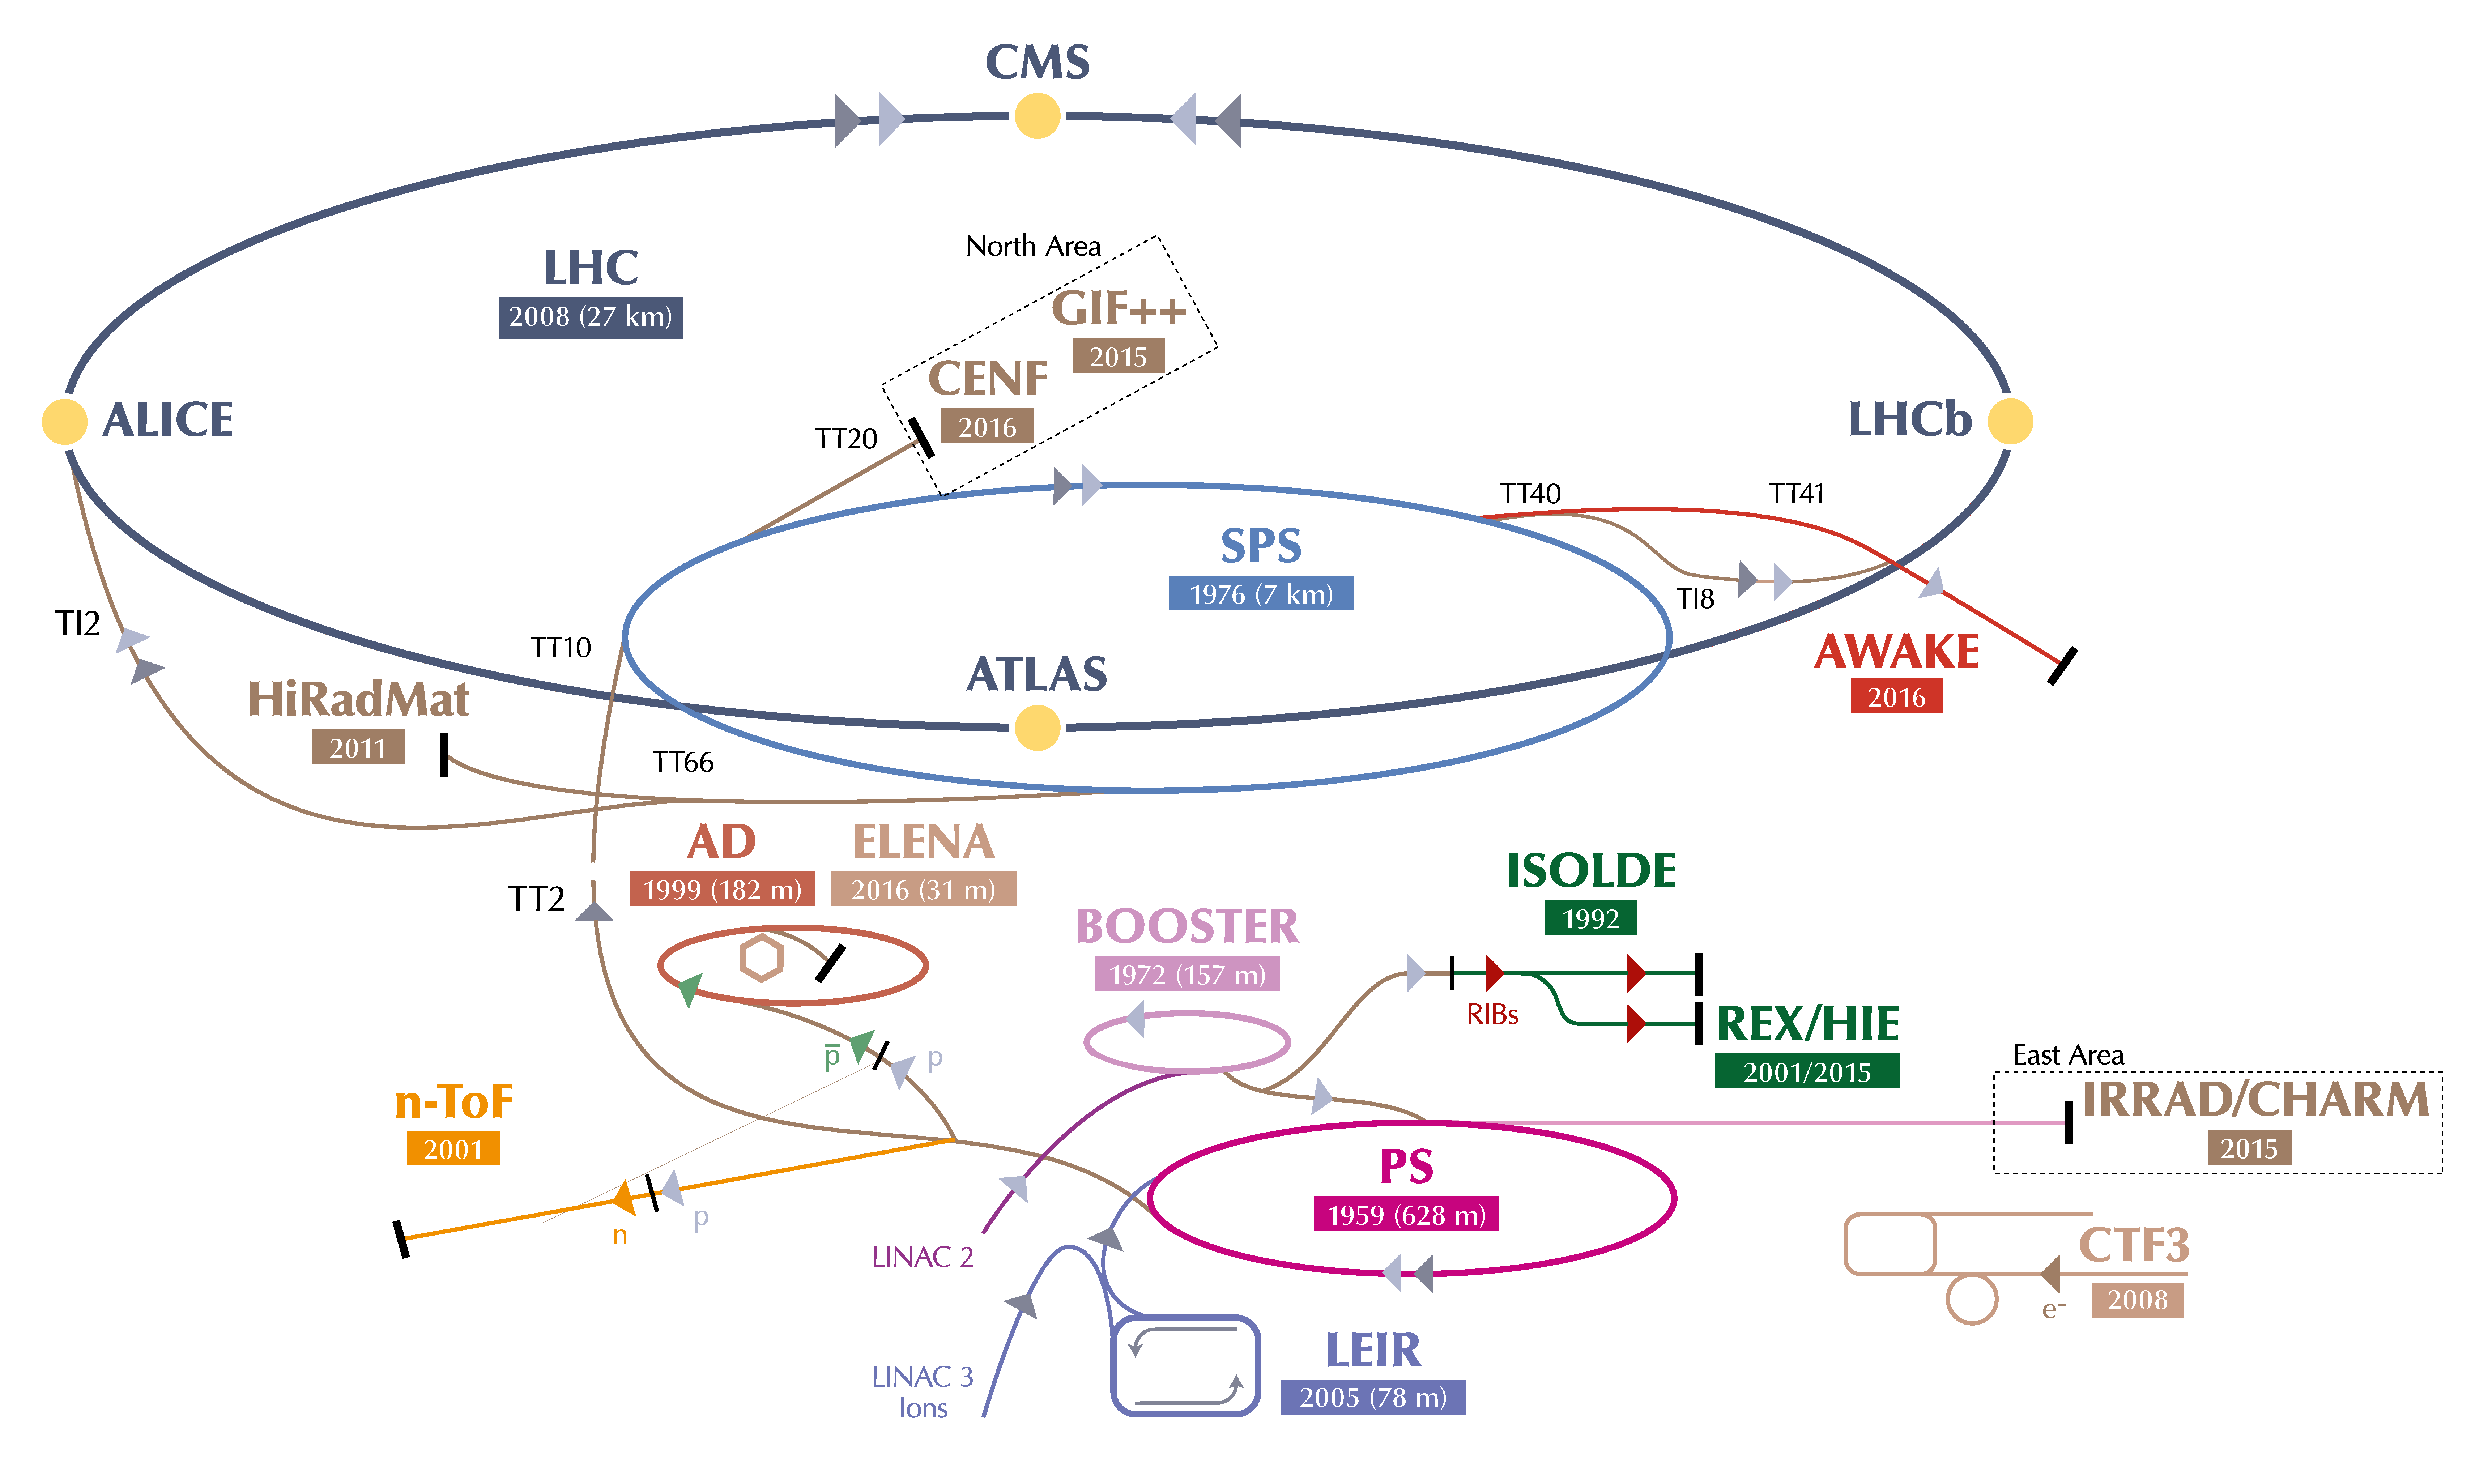
\includegraphics[width=0.99\linewidth,trim={20mm 0mm 20mm 0mm},clip]{figures/AcceleratorComplex}
    \caption{\label{Fig:WFA:AccComp} An overview of the CERN Accelerator Complex \cite{add:mobs:2016}.}
\end{figure}

% Intro paper \cite{caldwell:2009}
% Launch paper \cite{awake_collaboration:2014}
% Evolution paper \cite{caldwell:2016}
% Technical specs including simulation parameters \cite{gschwendtner:2016}
% Collaboration paper by Patric \cite{muggli:2017a}

% ================================================================================================================================ %
\section{Evolution of the Concept}
\label{WFA:History}

While AWAKE is the first proton driven wakefield experiment, a number of experiments with electron drive beams have confirmed the models produced by theory and simulations. The first experimental results of plasma wakefield acceleration were conducted at the Advanced Accelerator Test Facility at Argonne National Laboratory (ANL) outside Chicago, USA, and published in 1988~\cite{rosenzweig:1988}. The experiment split an electron beam of a few $\unit{nC}$ into a drive and a witness beam, and demonstrated that the drive beam generates accelerating wakefields as well as strong transverse fields. The accelerating gradient they produced was modest, only a few $\unit{MeV}$.

More recently, $\unit{GeV}$ level acceleration gradients have been achieved with an electron bunch at SLAC, where parts of a $42\unit{GeV}$ electron bunch saw energy doubling in an $85\unit{cm}$ plasma cell. The results were published in Nature in 2007~\cite{blumenfeld:2007}. The plasma stage produced a continuous spread in energy up to about $85\unit{GeV}$. However, only a small fraction of the charge was accelerated to these energies. The experiment later produced a discrete, accelerated bunch with a core of $74\unit{pC}$ in an accelerating gradient of $4.4\unit{GeV/m}$~\cite{litos:2014}.

Self modulation at FACET \cite{adli:2016}
Review by Patric \cite{muggli:2009}


% ================================================================================================================================ %
\section{AWAKE: A Design Overview}
\label{WFA:Design}

AWAKE is, as of the writing of this thesis, operational and in Run~1. The proton beam line arriving from the SPS joins with the laser beam and the electron beam line, and connects to a $10\unit{m}$ plasma stage. In addition, an electron source has been installed, and a new side tunnel had to be dug to fit the electron beam line connecting the source to the main assembly. Figure \ref{Fig:WFA:AWAKE} gives and overview of the experimental layout in the tunnel. The old CNGS target is still present, behind a shielding wall as it is highly radioactive. This, unfortunately, has created some constraints for fitting the downstream beam line and diagnostics, and may pose additional challenges for Run~2.

\begin{figure}[hbt]
    \centering
    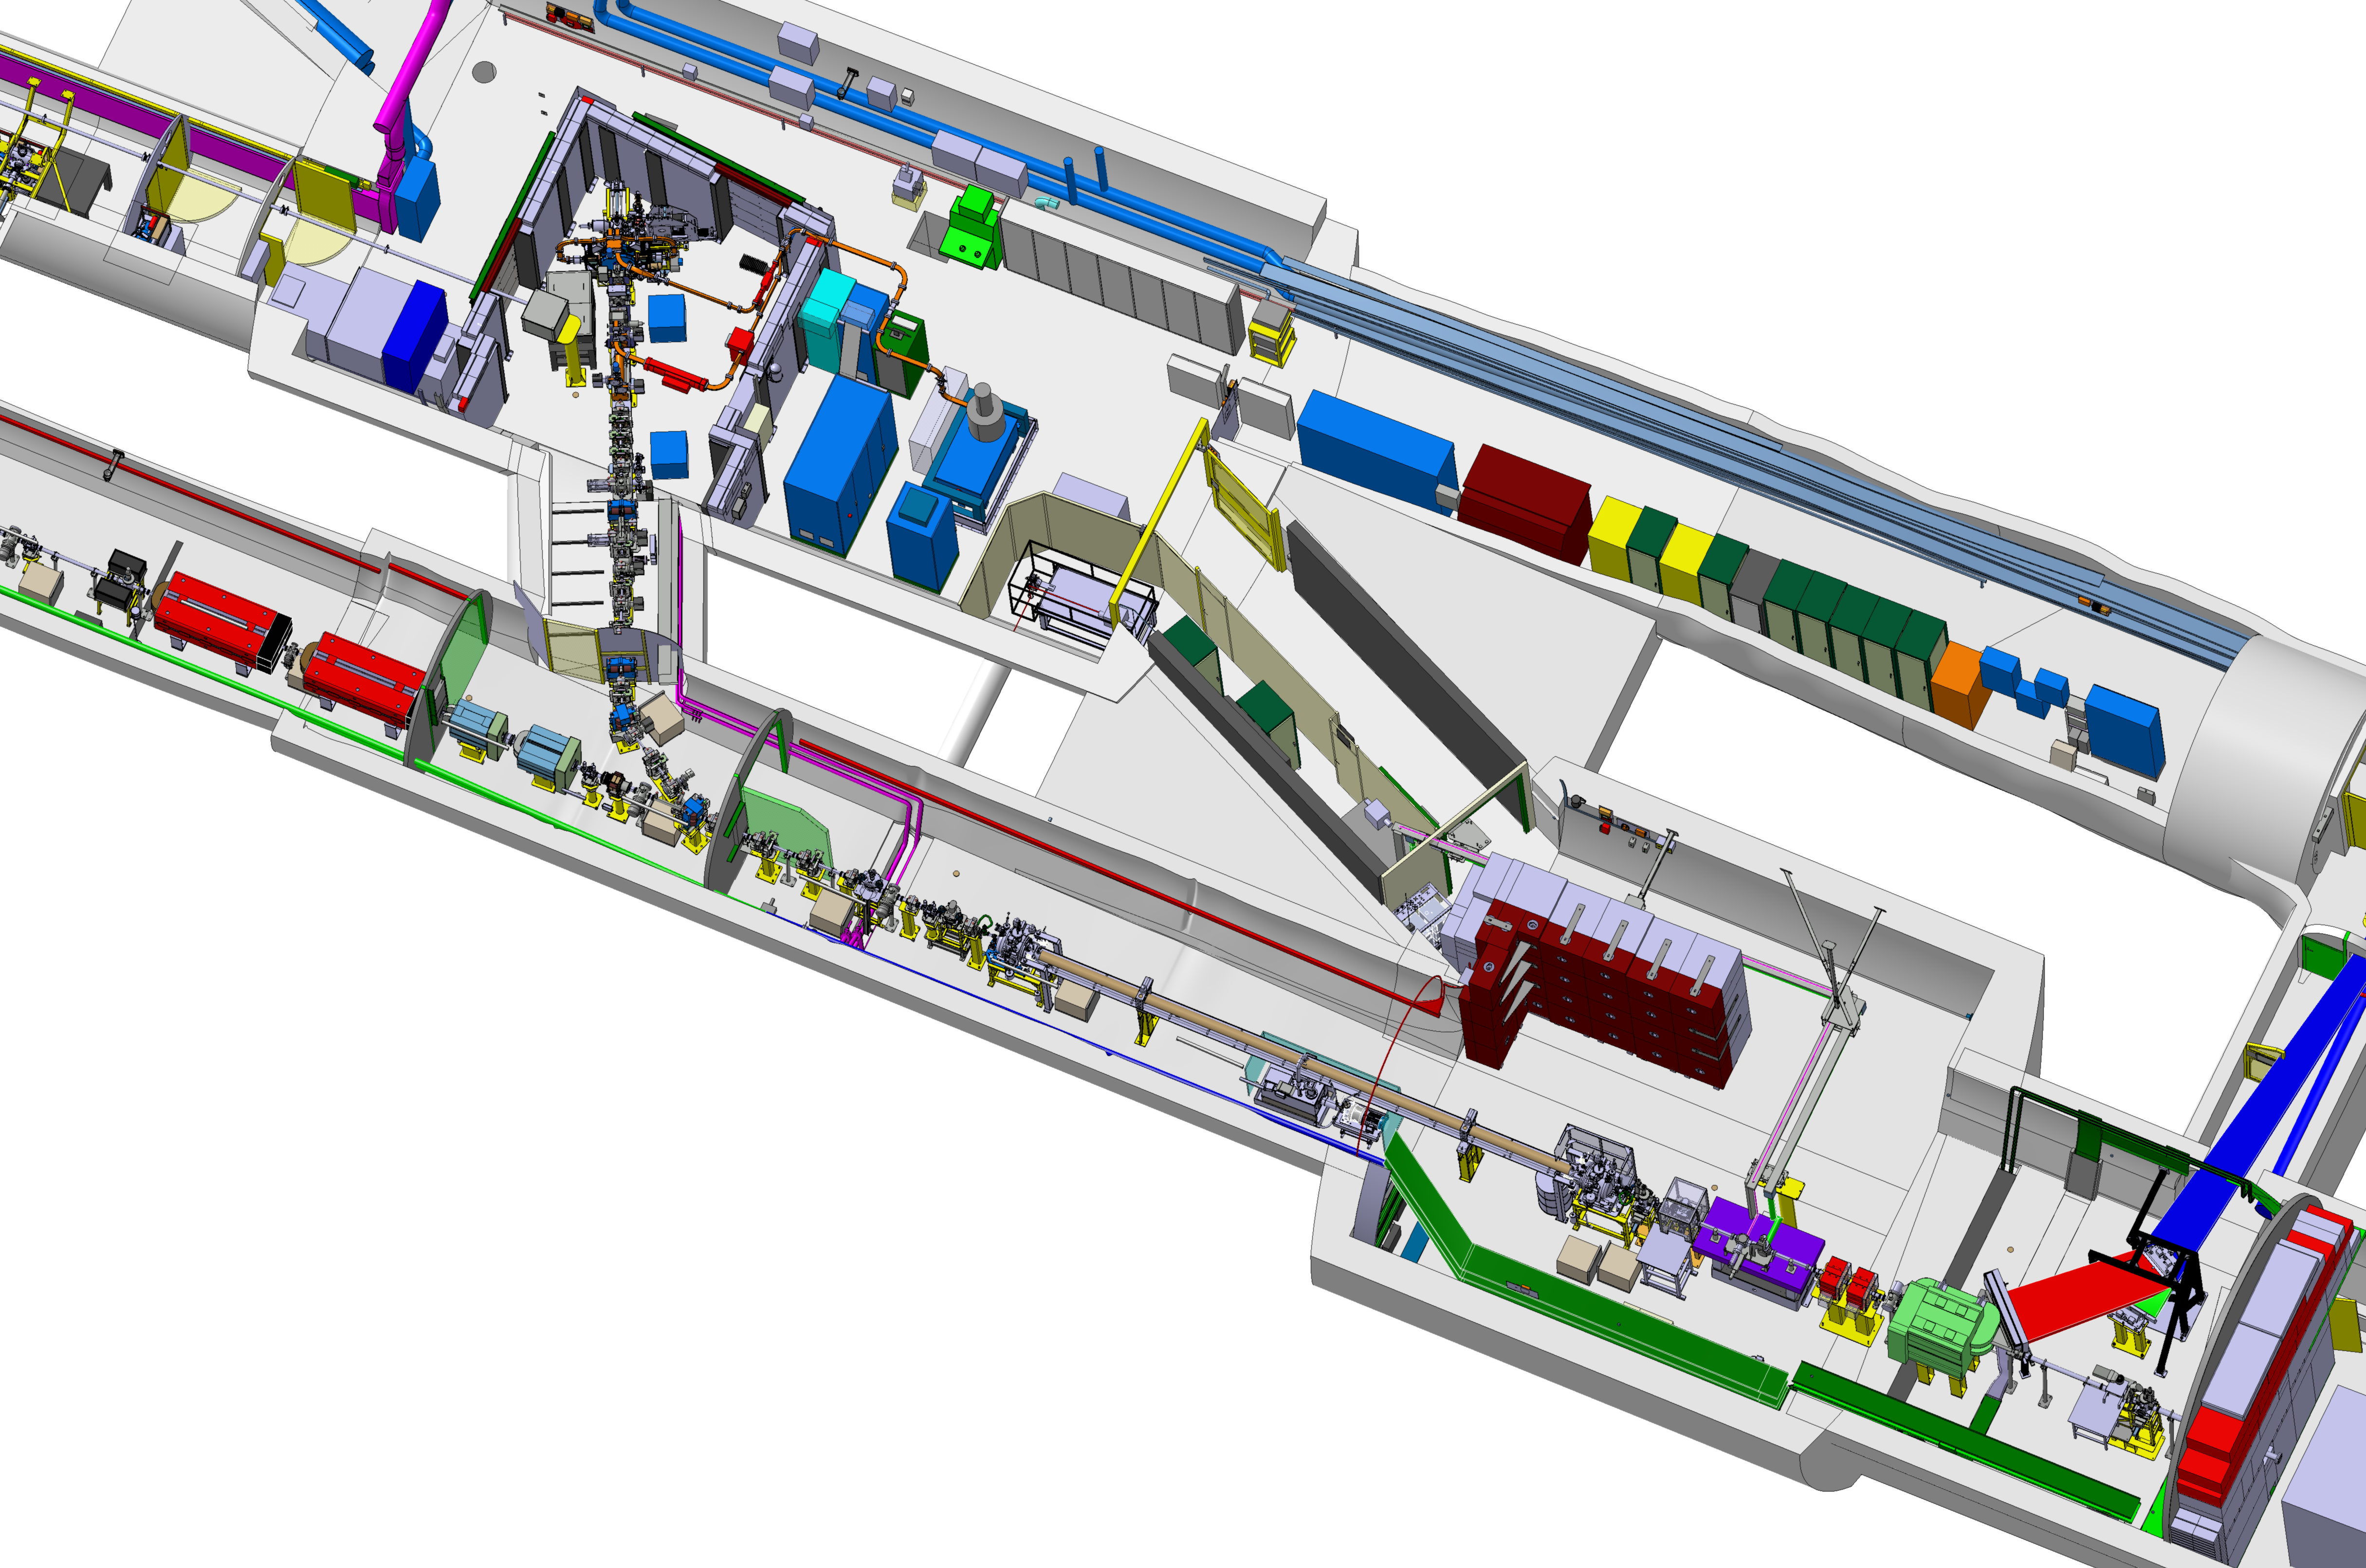
\includegraphics[width=0.99\linewidth,trim={0mm 0mm 0mm 0mm},clip]{figures/AwakeExperiment}
    \caption{\label{Fig:WFA:AWAKE} Drawing of the AWAKE experimental area with the key components labelled.}
\end{figure}

% ================================================================================================================================ %
\subsection{Plasma Source}
\label{WFA:Design:Plasma}

The requirements for the plasma source for AWAKE Run 1 were a $10\unit{m}$ long cell with a plasma electron density range of $1-10\nexp{14}\unit{cm}^{-3}$. The density variation should be within $0.2\%$, and the radius of the plasma channel should be $\geq 1\unit{mm}$. The plasma should also consist of heavy ions to mitigate ion motion \cite{caldwell:2015}.

\begin{figure}[hbt]
    \centering
    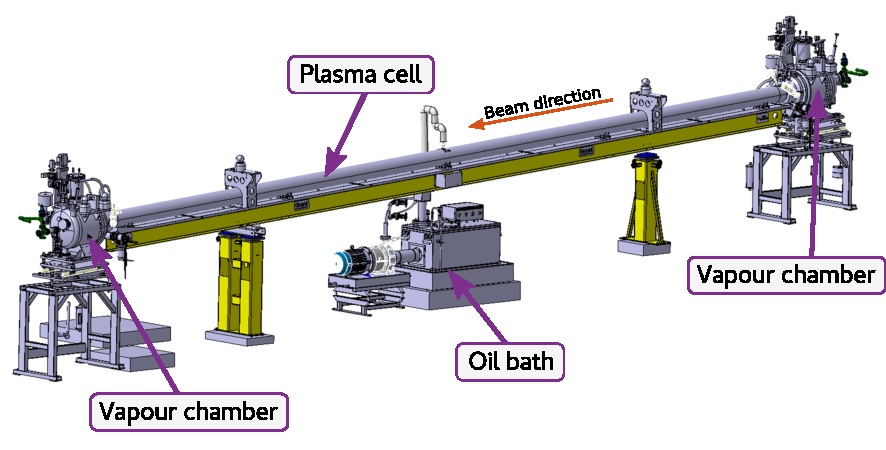
\includegraphics[width=0.99\linewidth,trim={0mm 0mm 0mm 0mm},clip]{figures/PlasmaCell}
    \caption{\label{Fig:WFA:PlasmaCell} A CAD drawing of the plasma cell and its related components, as presented in the 2016 AWAKE Status Report \cite{awake_collaboration:2016}.}
\end{figure}

For the AWAKE vapour source, rubidium (Rb) was chosen. Rubidium has a low melting point, $39.3\celsius$; a low first ionisation energy, $4.18\unit{eV}$; and a standard atomic weight of $85.47$. The plasma wavelength of rubidium ions with a $+1$ charge is roughly $400$ times that of the plasma electrons (see Eq. \ref{EQ:PWFA:L0W0}), preventing significant ion motion for AWAKE application \cite{vieira:2012a}. An additional benefit of using an alkaline metal like rubidium is that the second ionisation level is significantly higher, $27.3\unit{eV}$, making it relatively easy to prevent further ionisation and thus a lower charge/mass ratio \cite{awake_collaboration:2017}. The rubidium vapour is created by heating the reservoir and the plasma cell to around $150-230\celsius$ to reach the density range required for AWAKE \cite{caldwell:2015,muggli:2017a}.

The ionisation of the Rb vapour is achieved with a short laser pulse co-propagating with the proton drive beam. The laser can be timed such that the plasma channel is created inside the beam itself. The short laser pulse produces a sharp plasma edge that provides a good seed for the self-modulation instability \cite{vieira:2014a}. The section of the proton beam ahead of the laser does not interact strongly with the neutral rubidium vapour, although a low level of impact ionisation does occur. However, this effect is not significant \cite{awake_collaboration:2017}.

The ionisation laser used for AWAKE is a $780\unit{nm}$ Ti:Sapphire laser with a pulse length of $120\unit{fs}$ and a maximum compressed energy of $450\unit{mJ}$. The peak intensity is around $1.2\nexp{14}\unit{W/cm}^{2}$, with a spot size radius of $1\unit{mm}$ \cite{awake_collaboration:2017}. The appearance intensity needed for ionisation of rubidium is around $1.7\nexp{12}\unit{W/cm}^{2}$ \cite{augst:1989}. Ionisation of a second electron requires some $455$ times higher intensity, so we expect no secondary ionisation \cite{muggli:2017a}.

% ================================================================================================================================ %
\subsection{Electron Source}
\label{WFA:Design:ESource}

The AWAKE electron source needed for Run 1 consists of a $2.5$ cell RF-gun and a $1\unit{m}$ long booster structure, both operating at $3\unit{GHz}$, a cathode transfer chamber, beam diagnostics, and a beam transport line connecting it to the proton beam line. The beam is boosted to up to $20\unit{MeV}$ by a constant gradient acceleration structure. The RF-gun and the booster are powered by a $30\unit{MW}$ klystron \cite{awake_collaboration:2017,pepitone:2016}. Several of the components, including the RF-gun and klystron, were re-purposed from the former PHIN injector in the CLIC test facility \cite{chevallay:2012}. An overview of the electron source and the accelerating structure can be seen in Figure \ref{Fig:WFA:ESource}.

\begin{figure}[hbt]
    \centering
    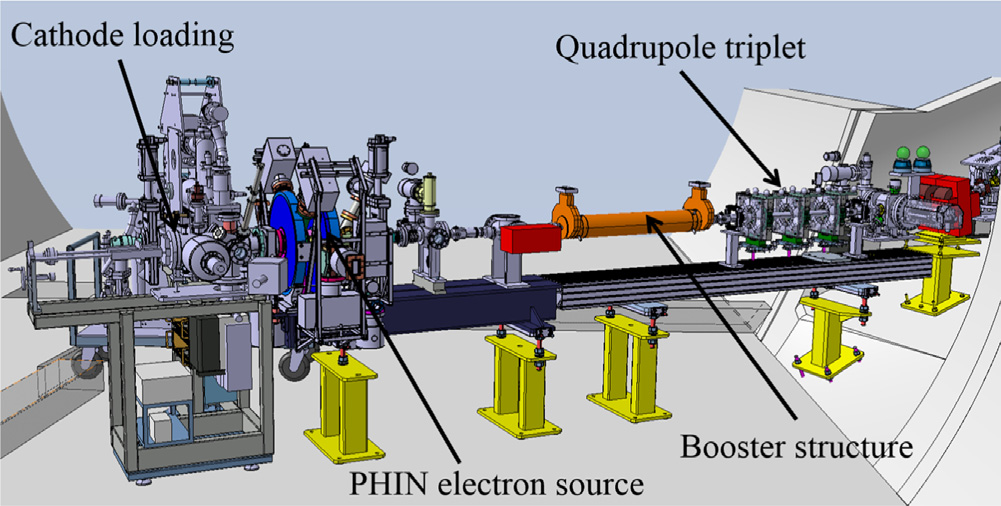
\includegraphics[width=0.70\linewidth,trim={0mm 0mm 0mm 0mm},clip]{figures/ElectronSource}
    \caption{\label{Fig:WFA:ESource} A CAD drawing of the electron source and accelerating structure \cite{pepitone:2016}.}
\end{figure}

% ================================================================================================================================ %
\section{Stages of the Experiment}
\label{WFA:AWAKE}

A summary of the AWAKE experiment

% ================================================================================================================================ %
\subsection{AWAKE Run 1}
\label{WFA:AWAKE:R1}

\begin{table}[hbt]
    \centering
    \caption{Nominal AWAKE experiment beam parameters for Run~1 \cite{gschwendtner:2014, gschwendtner:2016}.}
    \label{T:AWAKE-Run1}
    \begin{tabular}{lll}
        \rowcolor{tblhead}
        \texthh{Parameter}                    & \texthh{Proton Beam}          & \texthh{Electron Beam} \\
        \hline
        Momentum                              & $400\unit{GeV}$               & $16\unit{MeV}$ \\
        Charge                                & $4.8\unit{nC}$                & $200\unit{pC}$ \\
        Particles                             & $3\nexp{11}$                  & $1.25\nexp{9}$ \\
        Bunch length ($\sigma_{z}$)           & $12\unit{cm}\;(0.4\unit{ns})$ & $1.2\unit{mm}\;(4\unit{ps})$ \\
        Bunch size ($\sigma_{x,y}$)           & $200\unit{\mu m}$             & $250\unit{\mu m}$ \\
        Normalised emittance ($\emitN$)       & $3.5\unit{\mu m}$             & $2\unit{\mu m}$ \\
        Relative energy spread ($\Delta p/p$) & $0.035\%$                     & $0.5\%$ \\
        Beta function ($\beta^{*}_{x,y}$)     & $4.9\unit{m}$                 & $0.4\unit{m}$ \\
        Dispersion ($D^{*}_{x,y}$)            & $0$                           & $0$ \\
        \hline
    \end{tabular}
\end{table}

Description of Run 1. SMI, long e-beam.

% ================================================================================================================================ %
\subsection{AWAKE Run 2}
\label{WFA:AWAKE:R2}

Short e-beam, multiple stages, etc.

Problems relevant for this thesis.

Erik \cite{adli:2016a}

% ================================================================================================================================ %
\section{The Self-Modulation Instability in AWAKE}
\label{WFA:SMI}

Results from Run 1 of the experiment.

Karl \cite{rieger:2017}

Does the SMI require a seed? See muggli:2017 \cite{muggli:2017a}.

% ================================================================================================================================ %
